\documentclass{standalone}
\usepackage{tikz}
\usepackage{graphicx}
\usepackage{mathptmx}

\begin{document}

%%%%%%%%%%%%%
%% MODULES %%
%%%%%%%%%%%%%

\newcommand{\sinf}{
    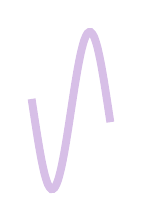
\begin{tikzpicture}
        % \draw[->,dashed,black] (-1,  0) -- (1, 0) node[right] {$t$};
        \draw[scale=0.5, domain=-1:1, smooth, variable=\x, purple!50!blue!25, line width = 0.1cm] plot ({\x}, {2*sin(2*pi*30*(\x))});
    \end{tikzpicture}
}

\newcommand{\expf}{
    
\begin{tikzpicture}
        % \draw[->,dashed,black] (-1,  0) -- (1, 0) node[right] {$x$};
        \draw[scale=0.5, domain=-1:1, smooth, variable=\x, purple!50!blue!25, line width = 0.1cm] plot ({\x}, {exp(\x)});
    \end{tikzpicture}
}

\newcommand{\timeseries}[1]{
    \begin{tikzpicture}
        \draw[scale=0.5,-,dashed,black] (-1,  0) -- (1, 0);% node[midway,below] {$t$};
        \draw[scale=0.5, domain=-1:1, variable=\x, black!10!white, mark=*, mark options={color=black}] plot ({\x}, {0.2*exp(2*sin(2*pi*50*(\x+#1)))});
    \end{tikzpicture}
}

\newcommand{\fittedo}[1]{
    \begin{tikzpicture}
        \draw[scale=0.5,-,dashed,black] (-1,  0) -- (1, 0);% node[right] {$t$};
        \draw[scale=0.5, domain=-1:1, smooth, variable=\x, red!75] plot ({\x}, {0.2*exp(2*sin(2*pi*50*(\x+#1)))});
    \end{tikzpicture}
}

\newcommand{\fittedp}[1]{
    \begin{tikzpicture}
        \draw[scale=0.5,-,dashed,black] (-1,  0) -- (1, 0);% node[right] {$t$};
        % \draw[scale=0.5, domain=-1:1, smooth, variable=\x, red] plot ({\x}, {0.75*(cos(2*pi*50*(\x+#1)))});
        \draw[scale=0.5, domain=-1:1, smooth, variable=\x, blue!75] plot ({\x}, {0.25*(cos(2*pi*50*(\x+#1)))*exp(2*sin(2*pi*50*(\x+#1)))});
    \end{tikzpicture}
}

\newcommand{\targetp}[1]{
    \begin{tikzpicture}
        \draw[scale=0.5,-,dashed,black] (-1,  0) -- (1, 0);% node[right] {$t$};
        \draw[scale=0.5, domain=-1:1, variable=\x, black!10!white, mark=*, mark options={color=black}] plot ({\x}, {0.75*(cos(2*pi*50*(\x+#1)))});
    \end{tikzpicture}
}

\newcommand{\dxdt}[1]{
    \begin{tikzpicture}
        \draw[scale=0.5,-,dashed,black] (-1,  0) -- (1, 0);% node[right] {$t$};
        \draw[scale=0.5, domain=-1:1, smooth, variable=\x, red, mark=*, mark options={color=black}] plot ({\x}, {0.25*(cos(2*pi*50*(\x+#1)))*exp(2*sin(2*pi*50*(\x+#1)))});
    \end{tikzpicture}
}

\newcommand{\sinhidden}[1]{
    \begin{tikzpicture}
        \draw[scale=0.5,-,dashed,black] (-1,  0) -- (1, 0);% node[right] {$t$};
        \draw[scale=0.5, domain=-1:1, smooth, variable=\x, black] plot ({\x}, {0.5*(sin(#1*4*pi*50*(\x)))});
    \end{tikzpicture}
}

\newcommand{\exphidden}[1]{
    \begin{tikzpicture}
        \draw[scale=0.5,-,dashed,black] (-1,  0) -- (1, 0);% node[right] {$t$};
        \draw[scale=0.5, domain=-1:1, smooth, variable=\x, black] plot ({\x}, {0.5*exp(#1*\x)});
    \end{tikzpicture}
}

\newcommand{\sensitivity}[1]{
    \begin{tikzpicture}
        \draw[scale=0.5,-,dashed,black] (-1,  0) -- (1, 0);% node[right] {$t$};
        \draw[scale=0.5, domain=-1:1, smooth, variable=\x, red] plot ({\x}, {#1*0.5*exp(0.1*\x)});
    \end{tikzpicture}
}

\newcommand{\contribution}[2]{
    \begin{tikzpicture}
        \draw[scale=0.5,-,dashed,black] (-1,  0) -- (1, 0);% node[right] {$t$};
        \draw[scale=0.5, domain=-1:1, smooth, variable=\x, red] plot ({\x}, {#1*0.5*exp(0.1*\x+#2) * 0.25*(cos(2*pi*50*(\x+#2)))*exp(2*sin(2*pi*50*(\x+#2)))});
    \end{tikzpicture}
}

\newcommand{\nnmodel}{
    \begin{tikzpicture}

        %% global params
        \def\lwd{0.2mm}
        \def\col{black!50}
        % \def\col{purple!50!blue!30}
        \def\alpha{0.75}
        \def\sizeNode{0.25cm}
        \def\colData{orange!10}
        \def\colfo{red!05}
        \def\colfp{blue!05}

        %% BOXES %%
        % \node [rectangle,minimum width=4.5cm,minimum height=6cm,fill,black!10] at (-1,0) {};
        % \node [rectangle,minimum width=4.5cm,minimum height=6cm,fill,black!10] at (-1+6,0) {};

        %% OBSERVATION MODEL 1 %%
        \def\oxi{-3}
        \def\oyi{1.5}
        %
        %% input
        \node [draw,fill,circle,minimum size=\sizeNode,inner sep=0pt,line width=\lwd,\col,label={left:{t}}] (oi1) at (\oxi,\oyi) {};
        %
        %% hidden
        \foreach \i\j in {\alpha/oh1,0/oh2,-\alpha/oh3}
        {
            \node [draw,fill,circle,minimum size=\sizeNode,inner sep=0pt,line width=\lwd,\col] (\j) at (\oxi+1,\oyi+\i) {};
        }
        \foreach \j in {oh1,oh2,oh3}
        {
            \draw[-,line width=\lwd,\col] (oi1.east) -- (\j.west);
        }
        \node [rotate=90,scale=0.7] () at (\oxi+1,\oyi+0.4) {$\dots$};
        \node [rotate=90,scale=0.7] () at (\oxi+1,\oyi-0.4) {$\dots$};
        %
        \foreach \i\j in {\alpha/0.1,0/0.25,-\alpha/0.5}
        {
            \node [fill,black!05,minimum height = 0.75cm] () at (\oxi+2,\oyi+\i) {\sinhidden{\j}};
        }
        %
        %% output
        \node [draw,fill,circle,minimum size=\sizeNode,inner sep=0pt,line width=\lwd,\col] (oo1) at (\oxi+3.75,\oyi) {};
        \foreach \i\j in {1*\alpha/oh1,0/oh2,-1*\alpha/oh3}
        {
            \node [line width=\lwd,\col] (\j) at (\oxi+2.75,\oyi+\i) {};
        }
        \foreach \i in {oh1,oh2,oh3}
        {
            \draw[-,line width=\lwd,\col] (\i.east) -- (oo1.west);
        }
        
        %% OBSERVATION MODEL 2 %%
        \def\oxi{-3}
        \def\oyi{-1.5}
        %
        %% input
        \node [draw,fill,circle,minimum size=\sizeNode,inner sep=0pt,line width=\lwd,\col,label={left:{t}}] (oi1) at (\oxi,\oyi) {};
        %
        %% hidden
        \foreach \i\j in {\alpha/oh1,0/oh2,-\alpha/oh3}
        {
            \node [draw,fill,circle,minimum size=\sizeNode,inner sep=0pt,line width=\lwd,\col] (\j) at (\oxi+1,\oyi+\i) {};
        }
        \foreach \j in {oh1,oh2,oh3}
        {
            \draw[-,line width=\lwd,\col] (oi1.east) -- (\j.west);
        }
        \node [rotate=90,scale=0.7] () at (\oxi+1,\oyi+0.4) {$\dots$};
        \node [rotate=90,scale=0.7] () at (\oxi+1,\oyi-0.4) {$\dots$};
        %
        \foreach \i\j in {\alpha/0.1,0/0.25,-\alpha/0.5}
        {
            \node [fill,black!05,minimum height = 0.75cm] () at (\oxi+2,\oyi+\i) {\sinhidden{\j}};
        }
        %
        %% output
        \node [draw,fill,circle,minimum size=\sizeNode,inner sep=0pt,line width=\lwd,\col] (oo1) at (\oxi+3.75,\oyi) {};
        \foreach \i\j in {1*\alpha/oh1,0/oh2,-1*\alpha/oh3}
        {
            \node [line width=\lwd,\col] (\j) at (\oxi+2.75,\oyi+\i) {};
        }
        \foreach \i in {oh1,oh2,oh3}
        {
            \draw[-,line width=\lwd,\col] (\i.east) -- (oo1.west);
        }
 
        %% PROCESS MODEL 1 %%
        \def\pxi{3}
        \def\pyi{1.5}
        %
        %% input
        \foreach \i\j\k in {0/p1i1/R}
        {
            \node [draw,fill,circle,minimum size=\sizeNode,inner sep=0pt,line width=\lwd,\col] (\j) at (\pxi,\pyi+\i) {};
        }
        %
        %% hidden
        \node [rotate=90,scale=0.7] () at (\pxi+1,\pyi+0.4) {$\dots$};
        \node [rotate=90,scale=0.7] () at (\pxi+1,\pyi-0.4) {$\dots$};
        \foreach \i\j in {\alpha/p1h1i,0/p1h2i,-\alpha/p1h3i}
        {
            \node [draw,fill,circle,minimum size=\sizeNode,inner sep=0pt,line width=\lwd,\col] (\j) at (\pxi+1,\pyi+\i) {};
        }
        \foreach \i in {p1i1}
        {
            \foreach \j in {p1h1i,p1h2i,p1h3i}
            {
                \draw[-,line width=\lwd,\col] (\i.east) -- (\j.west);
            }
        }
        %
        \foreach \i\j in {1*\alpha/0.1,0/0.25,-1*\alpha/0.5}
        {
            \node [fill,black!05,minimum height = 0.75cm] () at (\pxi+2,\pyi+\i) {\exphidden{\j}};
        }
        %
        %% output
        \node [draw,fill,circle,minimum size=\sizeNode,inner sep=0pt,line width=\lwd,\col] (p1o1) at (\pxi+3.75,\pyi) {};
        \foreach \i\j in {1*\alpha/p1h1f,0/p1h2f,-1*\alpha/p1h3f}
        {
            \node [] (\j) at (\pxi+2.75,\pyi+\i) {};
        }
        \foreach \i in {p1h1f,p1h2f,p1h3f}
        {
            \draw[-,line width=\lwd,\col] (\i.east) -- (p1o1.west);
        }

        %% PROCESS MODEL 2 %%
        \def\pxi{3}
        \def\pyi{-1.5}
        %
        %% input
        \foreach \i\j\k in {0/p2i1/R}
        {
            \node [draw,fill,circle,minimum size=\sizeNode,inner sep=0pt,line width=\lwd,\col] (\j) at (\pxi,\pyi+\i) {};
        }
        %
        %% hidden
        \node [rotate=90,scale=0.7] () at (\pxi+1,\pyi+0.4) {$\dots$};
        \node [rotate=90,scale=0.7] () at (\pxi+1,\pyi-0.4) {$\dots$};
        \foreach \i\j in {1*\alpha/p2h1i,0/p2h2i,-1*\alpha/p2h3i}
        {
            \node [draw,fill,circle,minimum size=\sizeNode,inner sep=0pt,line width=\lwd,\col] (\j) at (\pxi+1,\pyi+\i) {};
        }
                \foreach \i in {p2i1}
        {
            \foreach \j in {p2h1i,p2h2i,p2h3i}
            {
                \draw[-,line width=\lwd,\col] (\i.east) -- (\j.west);
            }
        }
        %
        \foreach \i\j in {1*\alpha/0.1,0/0.25,-1*\alpha/0.5}
        {
            \node [fill,black!05,minimum height = 0.75cm] () at (\pxi+2,\pyi+\i) {\exphidden{\j}};
        }
        %
        %% output
        \node [draw,fill,circle,minimum size=\sizeNode,inner sep=0pt,line width=\lwd,\col] (p2o1) at (\pxi+3.75,\pyi) {};
        \foreach \i\j in {1*\alpha/p2h1f,0/p2h2f,-1*\alpha/p2h3f}
        {
            \node [] (\j) at (\pxi+2.75,\pyi+\i) {};
        }
        \foreach \i in {p2h1f,p2h2f,p2h3f}
        {
            \draw[-,line width=\lwd,\col] (\i.east) -- (p2o1.west);
        }

        %% CROSS LINKS %% 
        \foreach \i\j in {p1h1i/p2h1i,p1h2i/p2h2i,p1h3i/p2h3i}
        {
            \draw[-,line width=\lwd,\col] (p1i1.east) -- (\j.west);
            \draw[-,line width=\lwd,\col] (p2i1.east) -- (\i.west);
        }

        %% TIME SERIES %%
        \def\x{-1}
        \def\y{4}
        \node [] () at (\x-1.5, \y) {
\includegraphics[width=2cm]{hare.pdf}};
        \node [] () at (\x-1.5,-\y) {
\includegraphics[width=2cm]{lynx.pdf}};
        \node [fill,\colData,label={above:{Time series (R)}}] () at (\x, \y) {\timeseries{0}};
        \node [fill,\colData,label={below:{Time series (N)}}] () at (\x,-\y) {\timeseries{2}};

        %% FITTED OBSERVATION MODEL ##
        \def\oxi{-3}
        \def\oyi{1.5}
        \node [fill,\colfo,label={below:{$\tilde{R}(t)$}}] () at (\oxi+5, \oyi) {\fittedo{0}};
        \node [fill,\colfo,label={above:{$\tilde{N}(t)$}}] () at (\oxi+5,-\oyi) {\fittedo{2}};

        %% DYNAMICS %%
        \def\xi{5}
        \def\yi{4}
        \node [fill,\colfo,label={above:{$\partial \tilde{R}/\partial t (t)$}}] () at (\xi, \yi) {\dxdt{0}};
        \node [fill,\colfo,label={below:{$\partial \tilde{N}/\partial t (t)$}}] () at (\xi,-\yi) {\dxdt{2}};

        %% FITTED PROCESS MODEL %% 
        \def\x{8}
        \def\y{1.5}
        \node [fill,\colfp,label={below:{$dR/dt(\tilde{R},\tilde{N})$}}] () at (\x, \y) {\fittedp{0}};
        \node [fill,\colfp,label={above:{$dN/dt(\tilde{R},\tilde{N})$}}] () at (\x,-\y) {\fittedp{2}};

        %% SIDE ARROWS %% 
        \def\x{2}
        \def\y{4}
        \def\lwd{0.3mm}
        \def\col{black!70}
        %
        \node [] (A) at (\x-2.0   ,  \y) {};
        \node [] (C) at (\x-0.25  ,  \y-1.5) {};
        \draw [-|,line width=\lwd,\col] (A) -| (C);
        %
        \node [] (A) at (\x+0.25  ,  \y-1.5) {};
        \node [] (C) at (\x+2.0   ,  \y) {};
        \draw [->,line width=\lwd,\col] (A) |- (C);
        %
        \node [] (A) at (\x-2.0   ,  -\y) {};
        \node [] (C) at (\x-0.25  ,  -\y+1.5) {};
        \draw [-|,line width=\lwd,\col] (A) -| (C);
        %
        \node [] (A) at (\x+0.25  ,  -\y+1.5) {};
        \node [] (C) at (\x+2.0   ,  -\y) {};
        \draw [->,line width=\lwd,\col] (A) |- (C);
        %
        \def\x{8}
        \def\y{4}
        \def\lwd{0.3mm}
        \def\col{black!70}
        %
        \node [] (A) at (\x-2.0  ,  \y) {};
        \node [] (C) at (\x-0.0  ,  \y-1.5) {};
        \draw [-|,line width=\lwd,\col] (A) -| (C);
        %
        \node [] (A) at (\x-2.0  ,  -\y) {};
        \node [] (C) at (\x-0.0  ,  -\y+1.5) {};
        \draw [-|,line width=\lwd,\col] (A) -| (C);

        %% LEGEND
        \node [scale=0.8] at (11,0)
        {
            \begin{tikzpicture}
                \def\x{0}
                \def\y{0.0}
                \def\dx{2}
                \def\col{purple!50!blue!30}
                \node [draw,fill,rectangle,\colData,minimum height=0.5cm,minimum width=1cm] at (\y,+3*\dx) {};
                \node [draw,fill,rectangle,\colfo,minimum height=0.5cm,minimum width=1cm]  at (\y,+2*\dx) {};
                \node [draw,fill,rectangle,black!05,minimum height=0.5cm,minimum width=1cm]  at (\y,+1*\dx) {};
                \node [draw,fill,rectangle,\colfp,minimum height=0.5cm,minimum width=1cm]  at (\y,+0*\dx) {};
                \draw [-|,black!70,line width=0.25mm] (\y-0.5,-1*\dx) to (\y+0.5,-1*\dx);
                \draw [->,black!70,line width=0.25mm] (\y-0.5,-2*\dx) to (\y+0.5,-2*\dx);
                \node [align=left] at (\y+2,+3*\dx) {Data time series};
                \node [align=left] at (\y+2,+2*\dx) {Interpolation};
                \node [align=left] at (\y+2,+1*\dx) {Hidden layers};
                \node [align=left] at (\y+2,+0*\dx) {NODE};
                \node [align=left] at (\y+2,-1*\dx) {Bayes. regul.};
                \node [align=left] at (\y+2,-2*\dx) {Differentiation};
            \end{tikzpicture}
        };

        % %% LEGEND
        % \node [scale=0.8] at (3,-6)
        % {
        %     \begin{tikzpicture}
        %         \def\x{0}
        %         \def\y{0.0}
        %         \def\dx{3}
        %         \def\col{purple!50!blue!30}
        %         \node [draw,fill,rectangle,orange!10,minimum height=0.5cm,minimum width=1cm] at (-2*\dx,\y) {};
        %         \node [] at ( -2*\dx,\y-1) {Response variable};
        %         \node [draw,fill,rectangle,black!05,minimum height=0.5cm,minimum width=1cm] at (-1*\dx,\y) {};
        %         \node [] at ( -1*\dx,\y-1) {Latent variable};
        %         \node [draw,fill,rectangle,green!10,minimum height=0.5cm,minimum width=1cm] at (0*\dx,\y) {};
        %         \node [] at ( 0*\dx,\y-1) {Process variable};
        %         \draw [-|,black!70,line width=0.25mm] (1*\dx-0.5,\y) to (1*\dx+0.5,\y);
        %         \node [] at ( 1*\dx,\y-1) {Regression};
        %         \draw [->,black!70,line width=0.25mm] (2*\dx-0.5,\y) to (2*\dx+0.5,\y);
        %         \node [] at ( 2*\dx,\y-1) {Differentiation};
        %     \end{tikzpicture}
        % };

    \end{tikzpicture}
}

%
%%%

%%%%%%%%%%
%% MAIN %%
%%%%%%%%%%

\begin{tikzpicture}
\node [scale=1] at (0,0) {
    \begin{tikzpicture}
        \node [scale=1] () at (0,0) {\nnmodel};
    \end{tikzpicture}
};
\end{tikzpicture}

%
%%%

\end{document}
